% !TeX root = ../thuthesis-caishiyu.tex

\chapter{研究背景综述}

本章节主要介绍本文的研究背景。本章节先介绍 NVM 存储介质的基本信息,使用方式以及编程难点。
接着介绍现有 NVM 工作中与本工作相关的工作,主要是 NVM 分配器以及 NVM 事务内存。
之后本章节将介绍目前的基于 NVM 的数据库管理系统,主要介绍本文所使用的存储引擎 N2DB。
然后本章节将介绍垃圾回收的背景,现有设计方法以及设计方法与 NVM 介质的适配性。
最后本章节将介绍数据恢复的相关工作,恢复原则,日志系统以及基于日志的系统的数据恢复流程。

\section{NVM 存储介质}

非易失性内存(NVM)是一种低延迟,字节寻址,大容量以及数据持久化的存储介质。
尽管 NVM 支持字节粒度的随机访问,但是实验证明,NVM 在以 64 字节粒度随机访问时读写性能最佳。
目前为止,市面上有两款商用化的 NVM 产品,分别是 NVMDIMM-N 以及 Intel Optane DC PMM(后简称 Optane)
NVMDIMM-N 同时采用了闪存以及 DRAM。上层应用可以直接访问 DRAM。
当系统断电时,数据会从 DRAM 复制到闪存中。为了保证数据能够在系统断电时执行数据复制,NVMDIMM-N 需要使用一个小型的备用电源。
Optane 使用了特殊的 3D XPoint 介质,不需要额外的备用电源。
Optane 的访问性能慢于 DRAM,但是其容量远大于传统的 DRAM。

\todo{找一下几个介质之间的数据对比}

NVM 的使用方式可以分为三种:(1)\textbf{文件系统模式}:文件系统模式指的是将 NVM 视为一个块存储设备,并且在上实现文件系统。上层的应用将数据以文件的形式存储在 NVM 上并且使用文件系统的读写接口访问 NVM 上的数据。(2)\textbf{内存模式}:内存模式指的是应用将 NVM 视为一块较大的内存。应用在使用 NVM 的过程中通过内存分配器来管理和使用该空间,并不会针对数据持久化性做额外的设计。(3)\textbf{DAX 模式}:DAX 模式的含义是直接访问模式。应用直接将 NVM 映射到自身的虚拟地址中一块区域。该模式允许应用直接使用内存访问的指令访问 NVM,绕过了文件系统,因此提高了访问性能。

使用 DAX 模式能够减少系统调用的次数,降低了访问开销。然而使用该模式意味着 NVM 对于应用不是透明的,应用需要手动管理 NVM 上的数据。
使用 DAX 模式在 NVM 上编程相较于在内存中编程有三个难点:

其一是 NVM 的数据管理需要保证空间分配和回收的持久化,而 DRAM 的数据管理不需要。
同时 NVM 的数据非易失意味着 NVM 上的内存泄漏问题也是持久化的,比 DRAM 中内存泄漏问题更为严重。

其二是 NVM 的数据持久化机制复杂。现有的计算机体系普遍使用缓存。当应用对 NVM 空间上数据进行更新,更新的数据会先修改缓存中的数据。此时数据的更新是易失的。当数据从缓存写回到 NVM 之前如果系统断电的话,则该数据丢失的。同时缓存的替换策略是编程者无法控制的。
因此编程者调用 Intel 架构下的缓存写回指令,如 clflush,clwb 指令,以确保数据顺利地写回到 NVM 上。
编程者还需要使用 fence 指令来保证指令不会乱序执行。

其三是 NVM 上数据结构的崩溃一致性问题。
NVM 仅能支持 8 字节的原子写,而是当对于一个数据结构的修改超过 8 个字节时,编程者就无法该修改的原子性,进而无法保证该数据结构始终保证一致性的状态。该问题有两个主流解决方法,分别是日志系统以及编程技巧。通过日志系统,应用可以将多个数据修改封装成一个事务,通过事务来保证多个数据更新的原子性。对于中止的事务,系统可以借助日志数据进行回滚,从而消除中止事务的片面影响,保证了数据结构的一致性。然而使用日志系统将会带来额外的开销。
另一种方法则编程者手动的管理数据结构的上数据更新的顺序,并且通过原子化修改一个标志位或者指针为来保证多个数据更新的原子性。该方法对于编程者而言更为困难,需要编程者谨慎设计所有数据更新的持久化时机以及顺序。
同时编程者需要频繁地调用缓存写回指令以及 fence 指令,而缓存写回指令和 fence 指令的数量会显著影响性能。因此如何尽可能地减少缓存写回指令以及 fence 指令是 NVM 领域的一大难题。

\section{NVM 相关研究}

NVM 的低延迟,持久化以及字节寻址等特性给内存分配器,事务内存,文件系统的设计带来了巨大的变化。这些相关工作在利用 NVM 的优异特性的同时,同样需要防止 NVM 存储空间内存泄漏以及保证 NVM 数据结构的崩溃一致性。
本章节将介绍两个 NVM 相关领域,NVM 分配器以及 NVM 事务内存,同时会介绍这些工作为了防止上述问题所采用的设计方法。

\subsection{NVM 分配器}

NVM 分配器与内存分配器一样,起到了管理,分配,回收存储空间的作用。
然而与内存分配器不同,NVM 分配器需要保证所有数据管理元数据的持久化,同时需要防范 NVM 空间的内存泄漏问题。

PMDK,是由 Intel 研发的 NVM 分配器\cite{pmdk}。
通常内存分配器支持两个接口,malloc 以及 free。
当应用需要内存空间时,使用 malloc 接口会得到分配器所分配的空间的地址,之后应用可以随意地使用该空间。
而 PMDK 的接口与内存分配器不同,其接口分别是 malloc-to 以及 free-from。
malloc-to 操作需要一个 NVM 地址作为输入。当应用调用 malloc-to 接口时,分配器会分配一块空间的空间,并且原子性地记录在输入的地址上。
PMDK 通过将分配空间和记录地址两个操作封装成一个事务来保证 malloc-to 操作的原子性。
因此 PMDK 可以保证所有分配的空间均是被使用的,即分配的空间的地址是被记录在 NVM 空间上。
PMDK 所采用的日志系统是写前日志,每个 malloc-to 需要在分配空间以及记录地址两个操作均记录一次日志。
相对于内存分配器,PMDK 的分配过程更加复杂,为了防止内存泄漏问题而引入了额外的日志开销。

Makalu\cite{bhandari_makalu_2016} 以及 Cai\cite{cai_understanding_2020} 采用了另外一种设计方法使得 NVM 分配器提供与内存分配器一样的接口,减少了上层应用编程的复杂性以及迁移的难度。
该设计方法允许 NVM 分配器能够无日志地分配和回收 NVM 空间。
NVM 分配器会在数据恢复阶段通过垃圾回收机制扫描 NVM 空间,以回收潜在的泄漏的空间。
Cai 在工作中将 NVM 上的数据结构描述为节点,各个节点彼此相连,形成一个图装结构。
所有不在图上的节点就被认为不被使用的,因此是潜在的泄漏的空间。
该工作为 NVM 分配器的恢复正确性给出了定义:一个 NVM 分配器是\textbf{可恢复的},当且仅当
分配器能够在数据恢复时将其元数据恢复到一个特定的状态。特定的状态指的是分配器的元数据中仅有被使用的空间才会被视为是已分配的。

使用日志的设计方法保证每一个分配和记录都是原子化的,但是其在运行时有额外的开销,同时在恢复时必须等到未提交的事务的影响消除后才能工作。
使用懒惰垃圾回收的设计方法在运行时的开销与内存分配器相差无几,同时恢复工作状态的所需的时间更短。
其缺点在于泄漏的空间会被回收不及时,以及只有扫描一种途径才能发现内存泄漏的空间。



\subsection{NVM 事务内存}

事务内存是被广泛研究的事务性系统。
内存上事务内存通过将对于一组内存上的读写封装成事务以保证该组读写的原子性,保证线程之间的隔离性。
NVM 上的事务内存起到与内存事务内存类似的作用,并且需要保证所有修改的持久化。
因此 NVM 上的事务内存研究采用日志系统来保证事务的原子性和持久化性。
NVM 事务内存的多数研究是在回滚日志或者重做日志之间进行性能上的取舍。

回滚日志记录的写操作的前象。每次事务进行写操作时之前,必须先将旧数据记录在回滚日志中并持久化,之后在原地址覆写上新的数据。事务每次读操作仅需要直接读取内存上的数据,因此读性能高。
然而每次写操作需要保证持久化顺序,因此写性能低。当事务内存恢复时,系统需要根据回滚日志中的数据回滚未提交事务的影响。


重做日志记录的是写操作的后象。一个事务的所有写操作会先合并并持久化到 NVM 上,之后再原地地应用在实际的内存地址上。因此在事务提交之后,NVM 空间中的数据不一定是最新的,其他事务可能需要读取重做日志以获得最新的数据。当事务内存恢复时,系统需要根据重做日志,重做所有提交事务的写操作。

NVM 数据库与 NVM 事务内存同样是事务性系统,同时也需要保证 ACID 四个事务特性。
因此 NVM 数据库理论上仅需要采用回滚日志以及重做日志中的一种就能保证数据是可恢复的。

\section{基于 NVM 的数据库管理系统}

现有许多工作致力于将 NVM 与数据库管理系统相结合。章节~\ref{ssec:nvmdb} 将根据设计思路介绍现有工作以及其瓶颈。章节~\ref{ssec:n2db} 将着重介绍本文所使用的 NVM 数据库存储引擎 N2DB 的基本信息以及组织结构。

\subsection{NVM 数据库现有工作及瓶颈}
\label{ssec:nvmdb}

现有 NVM 数据库相关工作根据设计思路可以分为三类,替换介质,局部重新设计以及整体重新设计。

\subsubsection{替换介质}

传统的数据库采用内存-磁盘的两层存储架构。
使用 NVM 替换磁盘或者内存是最为直观的设计思路。

\begin{figure}
    \centering
    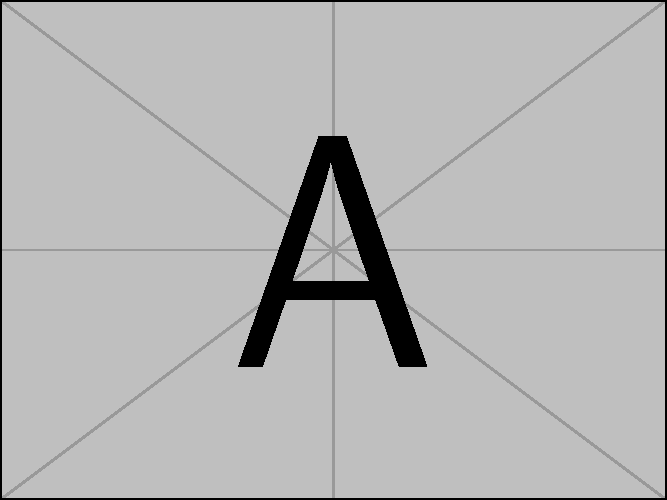
\includegraphics[width=0.6\linewidth]{example-image-a.pdf}
    \caption{常见的基于 NVM 的数据库的存储架构。\todo{参考 PPT 里的那个两层的图}}
    \label{fig:nvm-structure}
\end{figure}

Andy 等人通过 NVM 替换数据库的持久化介质,并为 NVM 上的数据存储格式进行细微的修改\cite{arulraj_lets_2015}。
模拟实验证明使用 NVM 代替磁盘能够带来 $1~2$ 倍的性能提升。

Katzburg 等人通过实验比较了关系型数据库在 NVMDIMM-N 上性能表现\cite{katzburg_nvdimm-n_2018}。
实验证明,Postgres 以及 SQLite 分别提升了 3.17 倍以及 1.79 倍。

DeBrabant 等人的工作表明,
基于 NVM 的文件系统的纯读写性能相对于 SSD 的读写性能能够提高三个数量级
\cite{debrabant_prolegomenon_2014}。然而将 MySQL,MongoDB 的底层文件系统从 SSD 替换成 NVM 文件系统后,仅能带来 1.5 倍 到 3 倍的性能提升。

从上述工作可以看出,NVM 相对于 SSD 的读写性能能提高三个数量级,但是关系型数据库系统的性能提升仅有 1 倍到 5 倍。因此简单地替换存储介质不足以全面利用 NVM 的硬件特性。
之所以关系型数据库的性能提升有限是由于关系型数据库中用于两个存储介质之间的数据同步以及数据管理开销大。
Harizopoulos 的工作中表明磁盘数据库中仅有 $14\%$ 的开销与事务相关,剩余的开销主要是数据同步以及数据管理带来的\cite{harizopoulos_oltp_2018}。内存数据库的事务的开销中有 $20\%$ 的开销是由日志系统以及持久化机制带来的。


\subsection{局部重新设计}

数据库管理系统中有许多组件,比如 SQL 执行引擎,事务引擎,记录数据存储,索引,分配器,垃圾回收,日志系统等。
一部分研究工作专注于将部分组件与 NVM 结合以获得局部的性能提升。

索引是一种广泛使用的数据结构,数据库中常见的索引有哈希表,B+ 树以及前缀树。
NVTree\cite{nv-tree} 是一个基于 NVM 的缓存友好型的 B+ 树。
NVTree 保证了崩溃一致性,同时通过降低 fence 指令的数量来提高索引的性能。
wB+Tree\cite{chen2015persistent} 也是一个基于 NVM 的 B+ 树。
该数据结构在运行时只使用原子写以及重做日志来就能保证各个树节点的崩溃一致性,
同时其性能相对于其他的持久化的 B+ 树提高了 8 倍到 27 倍。
ROART\cite{ma_roart_2021} 是基于 NVM 的前缀树。
其底层实现了一个无日志的分配器,同时通过节点的元数据的设计降低了数据恢复的开销。

Write-Behind Logging(WBL) 是一个基于 NVM 的数据库日志系统\cite{wbl}。
其在日志中不记录具体的事务操作,而记录了活跃事务的信息。
其相对于传统的日志系统,能够提高 $20\%$ 数据库的运行时性能,同时降低了数据库的恢复时间。

局部重新设计聚焦于数据库中的部分组件,以追求局部的性能提升。
此类设计思路仍然受限于传统数据库的内存和磁盘的双层架构。

\subsection{整体重新设计}

一些现有工作意识到上述两种设计思路的局限性,重新设计了数据库存储引擎。N2DB 采用了单层的存储架构,将所有的记录数据均存储在 NVM 上,并且基于多版本的记录存储实现了无日志的事务\cite{liu_graduate}。Zen 使用两层存储架构,将主要数据存储在 NVM 上,并且使用内存作为缓存。Zen 的实现也舍弃了日志系统,二者均显著提高了数据库的运行时性能,并且降低事务的延迟\cite{liu_zen_2021}。

\subsection{N2DB 简介}
\label{ssec:n2db}
本文的工作是在 N2DB 存储引擎中完成的。
N2DB 是一个基于 NVM 的零拷贝和无日志的数据库。表格数据仅存在在 NVM 上并且没有额外的拷贝,事务在运行时没有日志开销。
N2DB 使用多版本并发控制(Multi-Verion Concurrent Control,MVCC)来避免之间的事务冲突。基于 MVCC 的表格数据存储也是实现无日志的关键。
N2DB 的数据管理有两个粒度,分别是页粒度以及版本粒度。
因此 N2DB 上的垃圾回收以及数据恢复同样是两个粒度。

本章节将先介绍 N2DB 的存储引起结构,接着介绍 NVM 分配器,表格数据堆以及数据状态数组的数据结构。



\subsubsection{存储引擎组织架构}

如图~\ref{fig:n2db} 所示,N2DB 的架构整体上可以分为两层,下层是负责管理和分配 NVM 空间的 NVM 分配器。
上层通过接口向下层申请存储空间,其中有两个主要存储区域,分别是表数据堆以及事务状态数组。

\begin{figure}
    \centering
    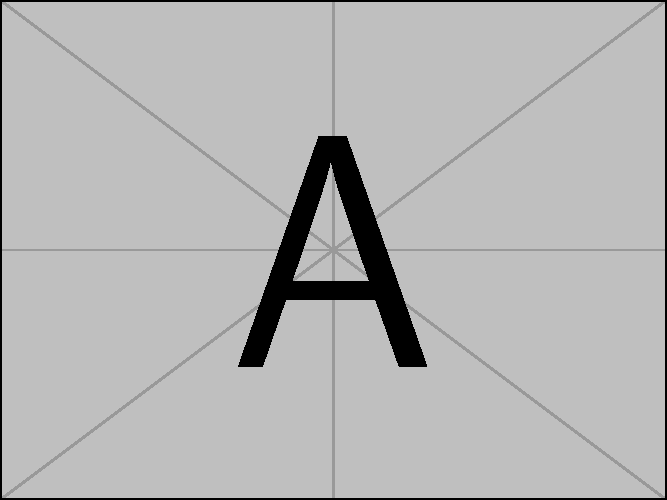
\includegraphics[width=0.6\linewidth]{example-image-a.pdf}
    \caption{存储引擎的架构示意图}
    \label{fig:n2db}
\end{figure}

\subsubsection{NVM 分配器}

\textbf{NVM 分配器:}NVM 分配器直接和 NVM 介质交互,并为上层的应用提供封装好的分配和回收接口。为了方便设计,N2DB 所使用的 NVM 空间通过 DAX 映射到一块连续的固定的虚拟地址上。
NVM 分配器以页粒度来分配和管理 NVM 存储空间。
N2DB 的默认页面大小设置为 2 MB。

如图~\ref{fig:n2db} 所示,NVM 分配器将整体的 NVM 空间分为了若干个页面。
第一个页面存储着 NVM 分配器的元数据。元数据中存放着一个用于记录页面分配情况的位图,页面所对应的比特为 1 时则说明该页面已经被分配,
比特为 0 则意味着该页面尚未被分配。
其他页面用于存储 N2DB 的数据。上层应用通过调用 NVM 分配器的分配接口申请数据所需的空间。

\subsubsection{表格数据堆}

一个表格可以有若干条记录,而这些记录会被物理地存储在表格数据堆中。
为了实现无日志的事务操作,N2DB 使用了基于 MVCC 的记录存储结构,即一个逻辑上的记录会物理地存在复数个版本。
每一条逻辑上的记录的所有历史版本都会物理地存放在表格数据堆中。
一个记录的所有的版本按照时间顺序会按照从新到旧顺序组织成一个链表形式,称之为版本链。其中有两种重要的数据结构,head 和 version。每一条记录有且仅有一个 head,而一个记录有多个 version。

记录的 head 是记录所对应的版本链的入口。
一个表格中的每一条记录都有一一对应的 ID,称之为 row\_ID。
因此每一个 head 也与 row\_ID 一一对应,系统可以通过 row\_ID 找到 head 的物理地址。
head 的数据结构定义如下:
\begin{itemize}
    \item 删除事务 ID(remove\_tx)用于记录删除该行的事务的事务 ID。事务 ID 是每个事务唯一的标识符。每个事务开始时都会向一个单调递增的计数器申请一个事务 ID。
    \item 垃圾回收次数(gc\_ts)是一个单调递增的计数器,代表了该行被垃圾回收的次数,通常用于防止同一 head 被重复回收。
    \item 最新版本(Newest\_version)记录了该记录最新的版本的地址。
\end{itemize}

记录的 version 用于存放记录的历史版本。
如图~\ref{fig:table} 所示,version 中除了该版本的历史数据以外还有其他元数据。Xmin 记录了创建该版本的事务的事务 ID,而 xmax 记录了废弃该版本的事务的事务 ID。
因此 xmin 和 xmax 可以指示一个 version 的生命周期,也就是 $[xmin, xmax)$,只有事务 ID 位于该区间的事务才有可能能够看到该 version。
Prev\_version 则是一个指向更早 version 的指针,如果一个 version 没有更早的 version,那么该成员变量的值应该为 null,即空指针。

一个表格需要向 NVM 分配器申请页面来存放 head 以及 version,而申请获得的页面的地址记录在 NVM 上,以防止内存泄漏。
如图~\ref{fig:table} 所示,一个表格的元数据中有两个页面的指针,这两个页面分别是 head pages 以及 version pages。
Head pages 是一个页面大小的指针数组,其中存放着该表格申请的用于存储 head 的页面的地址。
同理,version pages 也是一个指针数组,存放则用于存储 version 的页面的地址。
因此在重启之后,系统能够通过表格的元数据表格所申请的所有页面。

\begin{figure}
    \centering
    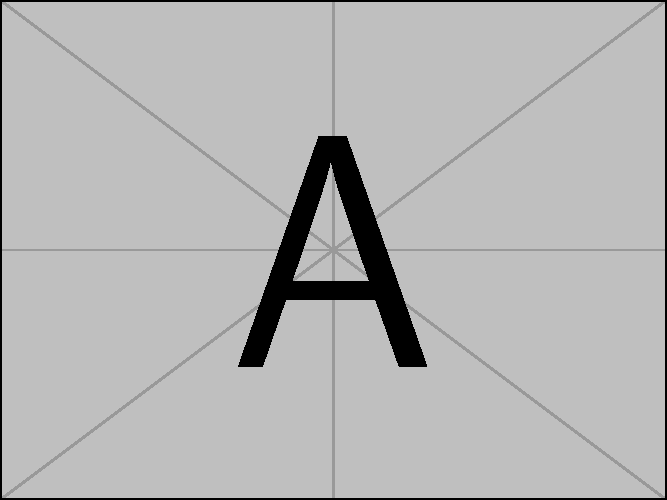
\includegraphics[width=0.6\linewidth]{example-image-a.pdf}
    \caption{表格的记录相关数据结构的组织结构。}
    \label{fig:table}
\end{figure}

\subsubsection{事务状态数组}

事务状态数组是一个逻辑上无限长的用于记录事务状态的数组。
每个事务一共有四种状态,分别是 INITIAL,IN-PROGRESS,COMMITTED 以及 ABORTED。
INITIAL 代表事务的起始状态。IN-PROGRESS 代表了事务正在处于运行状态。COMMITTED 意味着事务已经提交了,
而 ABORTED 代表了事务中止。
由于每个事务只有四种状态,因此每个事务只需要 2 比特。
虽然事务状态数组逻辑上是无限长的,但是在实际实现中,事务状态数组是一个固定大小的环形队列,具体的结构如图~\ref{fig:clog} 所示。
当事务状态的数量超过阈值之后,系统需要借助垃圾回收的信息来清理过期的事务的状态。

\begin{figure}
    \centering
    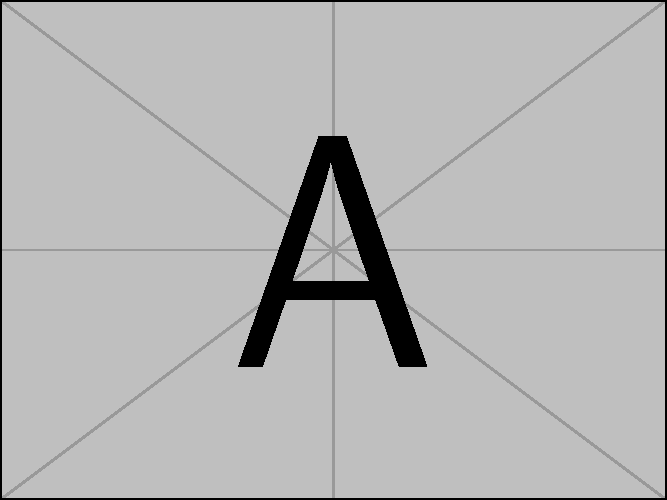
\includegraphics[width=0.6\linewidth]{example-image-a.pdf}
    \caption{事务状态数组的示意图}
    \label{fig:clog}
\end{figure}




\section{数据库的垃圾回收机制}

近十年来几乎所有的数据库管理系统均采用了 MVCC。
基于 MVCC 数据库管理系统在运行的过程中会不断产生需要回收的版本。这些版本不仅会对事务运行的性能产生影响,同时会占据存储空间。
因此 MVCC 数据库管理系统使用垃圾回收机制回收可回收的版本。
可回收的版本可以分为两类。
一类是任何后续事务都不会见到的版本。一个版本能否被另一个事务见到取决于另外一个事务的隔离级别以及时间戳。
另一类版本则是中止事务所创建的所有版本。
本章节将介绍数据库的垃圾回收的设计方法,并且分析各个设计方法在 NVM 上的适应性。

垃圾回收机制的需要解决三个问题,分别是如何发现可回收版本,回收可回收版本的粒度以及回收可回收版本的方法。

\subsection{发现可回收版本的途径}

事务所产生的不可见的版本位于版本链中,垃圾回收机制需要先发现可回收版本的位置信息才能回收。
发现可回收版本的途径可以分为三类,分别是后台清理(Background Vacuuming),合作清理(Cooperative Cleaning)以及事务信息。

后台清理指的是数据库有专门的扫描线程负责扫描所有页表的版本链,以发现潜在的可回收的版本。
为了降低后台扫描线程的扫描的开销,数据库系统会在表格数据中按照一定粒度维护脏位。
一个块表格数据如果脏位为 1,代表该区域最近被修改过,有潜在的可回收版本。
后台扫描线程被唤醒后只需要扫描脏位为 1 的区域,可以节省扫描的数据量。
使用后台清理的好处在于后台清理不会造成系统的吞吐率波动,同时系统可以通过增加后台扫描线程来调整垃圾回收的效果。Oracle\cite{oracle},Postgres\cite{pg} 以及 MySQL\cite{mysql} 是常见的采用后台清理的数据库管理系统。

合作清理指的是由事务来发现可回收的版本。事务在进行读,更新,删除等操作时,需要访问版本链。
当在访问版本链的过程中,事务不仅需要判断该版本对于事务自身的可见性,同时需要判断该版本对于全局的可见性。事务会将对全局不可见的版本的信息收集起来交由给垃圾回收机制,也可以由事务自身进行回收。
合作清理将扫描版本链的开销均摊到每个事务的执行。然而合作清理有两个弊端:一是版本链最好是从旧往新排列的,否则事务不容易访问到可回收的版本。二是不被访问到的记录就不会被回收,因此对于不均匀的负载不友好,一些记录的可回收版本将长期占据存储空间。采用该方法的主流数据库有 Hekaton\cite{hekaton}。

事务信息指的是事务根据事务自身进行的操作来判断潜在的可回收的空间。
与合作清理不同的是,事务信息指的是事务根据自身的操作类型,而不取决于自身所扫描过的版本的数量。
事务在进行更新操作时会创建出一个新的版本,当事务提交之后,旧数据所在的版本就是潜在的可回收的版本。
同理,事务删除一个记录并且提交之后,该记录所对应的版本链就是潜在的可回收的版本。
当事务结束时,事务可以将潜在的可回收的版本信息一并交给垃圾回收机制。
Hyper\cite{hyper} 采用的是该设计方法,并且 Hyper 针对该方法优化调整了数据库的存储结构。
Hyper 的数据库中的所有版本链均是从旧得新的。事务在进行更新时会复制一份旧版本,并将旧版本存放自己的一块连续空间中,称之为事务缓存。最后事务原地更新版本链最新的版本中的数据。
因此事务在提交时,事务缓存中所存放的版本均是潜在的可回收版本,并且这些版本的回收时机一致。
因此垃圾回收机制可以一次性回收一块连续的空间。

Andy 等人对于三种途径进行过性能对比测试\cite{mvcc_evaluation}。实验说明,不论是写偏向的负载还是读偏向的负载,采用事务信息方式的事务的平均性能比采用合作清理以及后台清理的平均性能高,但是波动更大。


\subsection{可回收版本的回收粒度}

可回收的回收粒度可以分为三类。
其中最细粒度的是元组粒度(Tuple-level),即垃圾回收机制以版本粒度来进行回收,后台清理和合作清理通常的回收粒度是元组粒度。
相对更粗的粒度称之为事务粒度(Transaction-level),即将一个事务相关的可回收版本一起清理。
而最粗的粒度为时间片粒度(Epoch-level),即将一个时间片中所有的事务视为一组,将一组事务相关的可回收版本一起清理。
由于传统数据库中内存与磁盘的延迟巨大,系统通常采用组提交(Group Commit)策略一次性提交一组事务来掩盖内存与磁盘之间的延迟差异。使用组提交的系统通常使用时间片粒度来清理可回收版本,例如 MySQL。

\subsection{可回收版本的回收频率}

可回收的回收频率指的是垃圾回收线程执行回收的频率。回收频率越高,系统中垃圾的数量就越少。
然而回收频率过高又会影响事务的性能。
回收频率可以分为两种情况。一类垃圾回收机制是由单独的回收线程来执行的,例如后台清理。回收的频率取决于该线程被唤醒的频率。
另一类垃圾回收机制是事务执行的一部分。
当一个线程执行完若干个事务后,垃圾回收机制就会被调用。
而两个垃圾回收之间所间隔的事务的数量就代表着垃圾回收的频率。
使用组提交的事务通常是在一组事务提交后进行回收。

\subsection{NVM 数据库的垃圾回收设计的变化}

基于 NVM 的数据库回收机制相较于传统的数据库管理系统有两个设计上的挑战。

一是垃圾回收元数据的持久化。大部分内存数据库管理系统会在内存中保存一个版本的空闲队列。
当表格需要新版本则从空闲队列中取得一个版本,当表格回收一个版本时需要将该版本添加到空闲队列。
空闲队列记录了版本的分配信息,然而内存中的版本分配是不需要考虑版本分配信息的持久化的,而 NVM 数据库则需要考虑该问题。
NVM 数据库有两个设计的方向,一是将空闲队列持久化,二是使用别的持久化数据结构来记录版本分配信息。两个方法均要么通过日志保证该元信息的数据结构的任何方法均是原子性的,要么针对性设计出恢复方法。

二是垃圾回收机制需要保证版本链的崩溃一致性。垃圾回收机制也需要和事务一样经常访问版本链,
同时需要对版本链上的版本进行操作,比如将指定版本从版本链上断开。
垃圾回收机制需要对于版本链上的指针操作的顺序针对性设计,以防止版本链的不一致。

基于 NVM 的数据库的垃圾回收机制同样有一个主要的优势,即组提交在 NVM 上是没必要的。
组提交是传统数据库由于内存和磁盘性能差异过大而做的妥协。基于 NVM 系统的数据库管理无需组提交,因而不需要比事务粒度更粗的垃圾回收粒度,进而可以降低垃圾回收机制对于性能产生的波动。


\section{数据库的数据恢复机制}

数据库系统在运行的过程中,有可能会发生硬件故障,软件故障,网络错误以及操作系统故障。
数据库管理系统需要防范故障的发生,同时要在故障发生之后能够将系统迅速地恢复到正常的工作状态。数据恢复机制是为了系统遇到非硬件故障设计出的。
主流的数据恢复机制是使用写前日志(Write-Ahead Log,WAL)。
采用写前日志的数据库管理系统会将一个事务中的所有操作均记录在日志文件中,
事务提交前会先将该事务对应的日志持久化,之后提交。
事务在中止后也可以根据日志回滚事务的操作。
本章节将介绍数据库的数据恢复机制的原则,之后介绍写前日志系统的基本情况,最后介绍主流的基于日志系统的恢复策略,即 ARIES。

\subsection{数据恢复的原则}

数据库管理系统是一个事务性的系统,因此数据库中的事务需要保证 ACID 四个特性。
数据库恢复机制需要尤其保证事务的原子性以及持久化。
原子性(Atomic)意味着一个事务的所有操作所造成的影响要么都存在,要么都不存在,不存在片面的状态。
持久化(Durability)意味着所有提交事务的影响不会因为故障而消失。
因此数据库管理系统需要将提交事务的影响以某种形式持久化到持久化介质上。

当系统遭遇故障并且重启时,系统中可能存在未提交事务的影响,比如说未提交事务更新所创造的版本,未提交事务修改表格的元数据。同时提交事务的修改可能尚未被持久化到持久化机制中,或者表格数据中并不存在提交事务的修改。因此数据库的数据恢复机制需要这几种异常情况。

综上所述,数据库管理系统的数据恢复机制需要严格满足两条基本的原则:
\begin{enumerate}
    \item 所有提交事务的影响均持久化。
    \item 所有未提交事务的影响必须被消除。未提交的事务包括中止事务以及因为故障而中断的事务。
\end{enumerate}


\subsection{日志系统简介}

日志系统的作用是用于记录事务的操作,并且将事务的操作记录在日志文件中并且进行持久化。
日志文件中是一个仅能顺序添加的文件。
事务的每一个操作均对应一个日志条目。
每一条日志均有一个全局唯一的日志序列码(Log Sequence Number)。
日志条目中一般会记录事务操作的前象以及后象。
仅记录前象的日志称之为回滚日志(Undo Log),而只记录后象的日志称之为重做日志(Redo Log)。
一个日志条目的数据结构定义如下:
\begin{itemize}
    \item 日志序列码(Log Sequence Number,LSN):日志序列码是每一个操作唯一的标识符,事务在生成日志条目时需要向一个中心化的计数器获取每个操作对应的日志序列码。一个事务的所有操作的日志序列码都是按照先后顺序严格递增的。
    \item 事务 ID(Transaction ID):事务 ID 是每个事务唯一的标识符。不同事务系统中的事务 ID 的生成方法各不相同。
    \item 表格 ID(Table ID):表格 ID 为该事务所操作的表格的标识符。
    \item 操作类型(Log Record Type):日志条目的操作类型记录了该事务的操作类型,包括更新,删除,插入等。
    \item 页 ID(Page ID):该操作所涉及的页面标识符。
    \item 重做数据(Redo):重做数据中记录该操作更新之后的数据。
    \item 回滚数据(Undo):回滚数据中记录该操作更新之前的旧数据。
    \item 前驱操作的日志序列码(Previous LSN):前驱操作的日志序列码记录着该操作在同一个事务中的前驱操作的日志序列码。一个事务的操作在日志上并不一定连续。事务在回滚时可以根据这成员变量倒叙遍历所有事务的操作,不要扫描日志文件。
\end{itemize}


数据库管理系统在记录日志文件之外,还会定期将内存中的脏页写回到磁盘上。
数据库将脏数据写回到磁盘的操作称之为制造检查点。
同时数据库会将日志文件中记录一次制造检查点操作。
图~\ref{fig:wal} 中展示一个 WAL 日志文件示例。从图中可以看出,事务 1 执行了两个更新操作,事务 2 执行了一个插入操作,之后系统执行了一次检查点操作。当检查点操作之后,事务 1 提交了。
事务 3 执行了删除操作,最后系统故障。


\begin{figure}
    \centering
    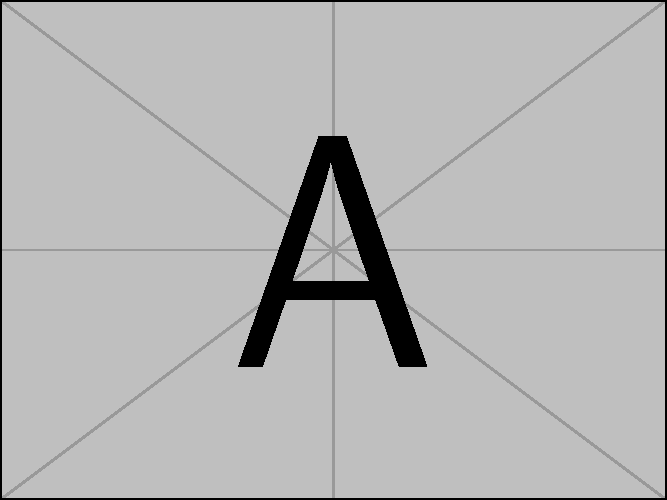
\includegraphics[width=0.6\linewidth]{example-image-a.pdf}
    \caption{WAL 示例}
    \label{fig:wal}
\end{figure}

\subsection{基于写前日志的事务运行时流程}

当事务创建时,其会向系统申请一块连续的空间用于存储该事务的所有操作对应的日志条目。当事务执行任何一个操作时,该事务都会添加一条对应的日志条目,并且获取对应的日志序列码。对于插入和更新操作,日志条目中的重做数据中会记录所插入的新记录的数据或者所更新的数据。对于更新和删除操作而言,回滚数据中记录了更新前的数据以及删除前的数据。

在事务提交之前,系统会先将日志刷到持久化介质上。之后数据库管理系统会认为该事务已提交。由于事务会频繁地产生日志条目,并且将数据刷到持久化介质延迟很大,因此数据库管理系统采用组提交方法来均摊一个事务刷日志的延迟。
但是组提交会降低单个事务的平均延迟。

当事务的日志刷到持久化介质之后,事务日志中的更新就可以先应用到内存中的表格数据中。内存中的表格数据始终领先于持久化数据上的表格数据。
由于日志文件的长度有限,当日志文件满时,系统将会从内存向内存刷写表格数据,同时在日志文件中记录一次检查点操作。
由于磁盘文件是按照页粒度管理的表格文件的,内存中的表格数据会按照页粒度刷写到持久化介质上,
各个页面所刷写的时刻就不会完全一致。
因此数据库管理系统会在各个页面的元数据记录该页面上最新的操作所对应的日志序列码。
数据恢复可以根据各个页面上的元数据针对性恢复。


\subsection{基于日志系统的数据恢复流程}

日志文件记录了事务的操作,而数据库可以根据日志文件进行数据恢复。
ARIES 是最主流的基于写前日志的数据恢复方法。ARIES 最早于 1999 年由 C.Mohan 所提出\cite{mohan_aries_1992}。

\begin{figure}
    \centering
    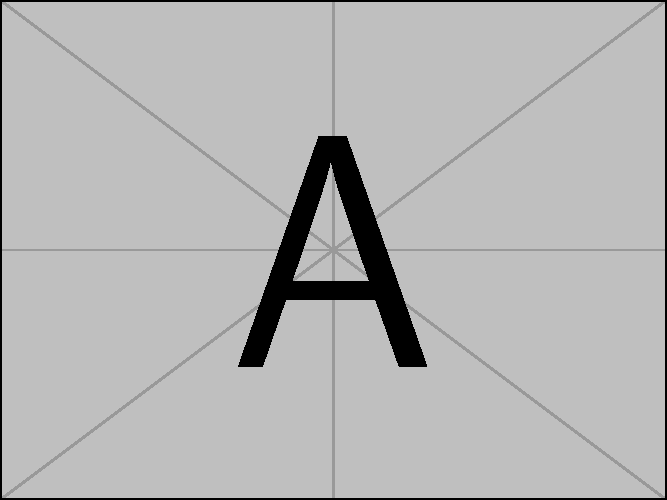
\includegraphics[width=0.6\linewidth]{example-image-a.pdf}
    \caption{ARIES 恢复流程}
    \label{fig:ARIES}
\end{figure}


图~\ref{fig:ARIES} 中展示了简化的 ARIES 的恢复流程以及各个流程涉及的日志条目范围。
ARIES 的数据恢复流程可以分为三个阶段,分别是分析,重做以及回滚。

\textbf{分析阶段:}重启之后首先扫描最新的日志文件,直到找到最新的一个检查点。之后系统会记录所有在检查点至系统故障时时处于活跃的事务信息,以及这些事务相关操作。
对于磁盘数据库而言,系统可以根据页面上记录的最新日志序列码来判断该日志文件是否最新的。

\textbf{重做阶段:}系统在收集完所有活跃事务的信息之后,系统将所有活跃的所对应的操作按照日志顺序重做。当系统完成所有重做操作之后,记录数据的状态将与系统宕机时最后一个日志条目所对应的状态一致。

\textbf{回滚阶段:}最后系统将所有事务所对应的操作从新到旧回滚,同时所有回滚所执行的操作也需要记录日志,以防止系统在此时宕机造成了回滚操作的丢失。
以图~\ref{fig:wal} 为例,系统将事务 2 的插入操作以及事务 3 的删除操作进行回滚,同时在日志中新添加了两条回滚操作的日志。当系统完成了回滚阶段之后,数据库管理系统就能正常地提供服务。

采用 MVCC 的数据库管理系统的数据恢复方法有两个不同。首先,日志条目中只记录后象的位置,不需要记录实际的数据。
其次,MVCC 的数据库管理系统支持快照隔离(Snapshot Isolation),事务在运行时会直接忽略未提交的事务所进行的修改。因此恢复过程中的回滚阶段也没有必要,但是未提交事务所创建的不可见版本仍需要回收。






